%% Monte Carlo in Movie Production: Ray Tracing and Sampling

%% REMOVEME
%% Ще говоря за това как ползваме алгоритми, някои от които учат в университета
%% или изборни курсове (напр. курса "Трасиране на лъчи" на Веселин Георгиев) на
%% практика за създаване на филми. Ще обясня накратко какво представлява
%% трасирането на лъчи, няколко алгоритъма за global illumination integration,
%% какво е метода Monte Carlo и защо е подходящ, как различни sampling методи
%% влиаят на финалния резултат и защо, както и няколко конкретни sampling
%% дизайни.

\documentclass[pdf]
{beamer}
\usepackage{outlines}
\mode<presentation>{\usetheme{}}
\title{Monte Carlo in Movie Production}
\subtitle{Ray Tracing and Sampling}
\author{Slavomir Kaslev \\
  \href{mailto:slavomir.kaslev@gmail.com}{slavomir.kaslev@gmail.com}}
\begin{document}

\begin{frame}
  \titlepage
\end{frame}

\begin{frame}{About me}
  \begin{itemize}
    \pause
  \item My name is Slavomir Kaslev
    \pause
  \item Software engineer
    \pause
  \item I work at Worldwide FX as Head of R\&D
  \end{itemize}
\end{frame}

\begin{frame}{About Worldwide FX}
  \begin{itemize}
    \pause
  \item Founded in 2001
    \pause
  \item The first VFX studio in Bulgaria
    \pause
  \item $\sim 250$ visual artists
    \pause
  \item More than 115 feature film projects completed
  \end{itemize}
\end{frame}

\begin{frame}{Studio demo reel}
\end{frame}

\begin{frame}{Software we use}
  \begin{itemize}
    \pause
  \item Linux on workstations, farm nodes and servers
    \pause
  \item Mac OS and Windows on some workstations
    \pause
  \item Avid, Blender, Mudbox, Mari, Maya, Houdini, Katana, RenderMan, Nuke, RV, Massive, Photoshop, Unity, ZBrush, 3DEqualizer, ...
    \pause
  \item In-house tools
    \pause
  \item ``Software is eating the world'' \pause Why? \pause Hint: Dependent Types
  \end{itemize}
\end{frame}

\begin{frame}{Rendering}
  \begin{itemize}
    \pause
  \item Renderer is a software that generates an image from 3D scene description
    \pause
  \item 3delight, Arnold, RenderMan, V-Ray, mental ray, Maxwell, Redshift, etc
    \pause
  \item Open source: Cycles, pbrt, appleseed, Mitsuba, LuxRender, etc
    \pause
  \item In-house: Hyperion at Disney, Manuka at Weta Digital, Plume at ILM, Blue Sky, etc
    \pause
  \item Ray tracing won at least in the movie industry. \pause Why?
    \pause
    Computer time is cheap, people time is expensive.
    \pause
  \item ``Physically Based Rendering: From Theory to Implementation'' by Matt Pharr and Greg Humphreys
  \end{itemize}
\end{frame}

\begin{frame}{Bussiness card ray tracer}
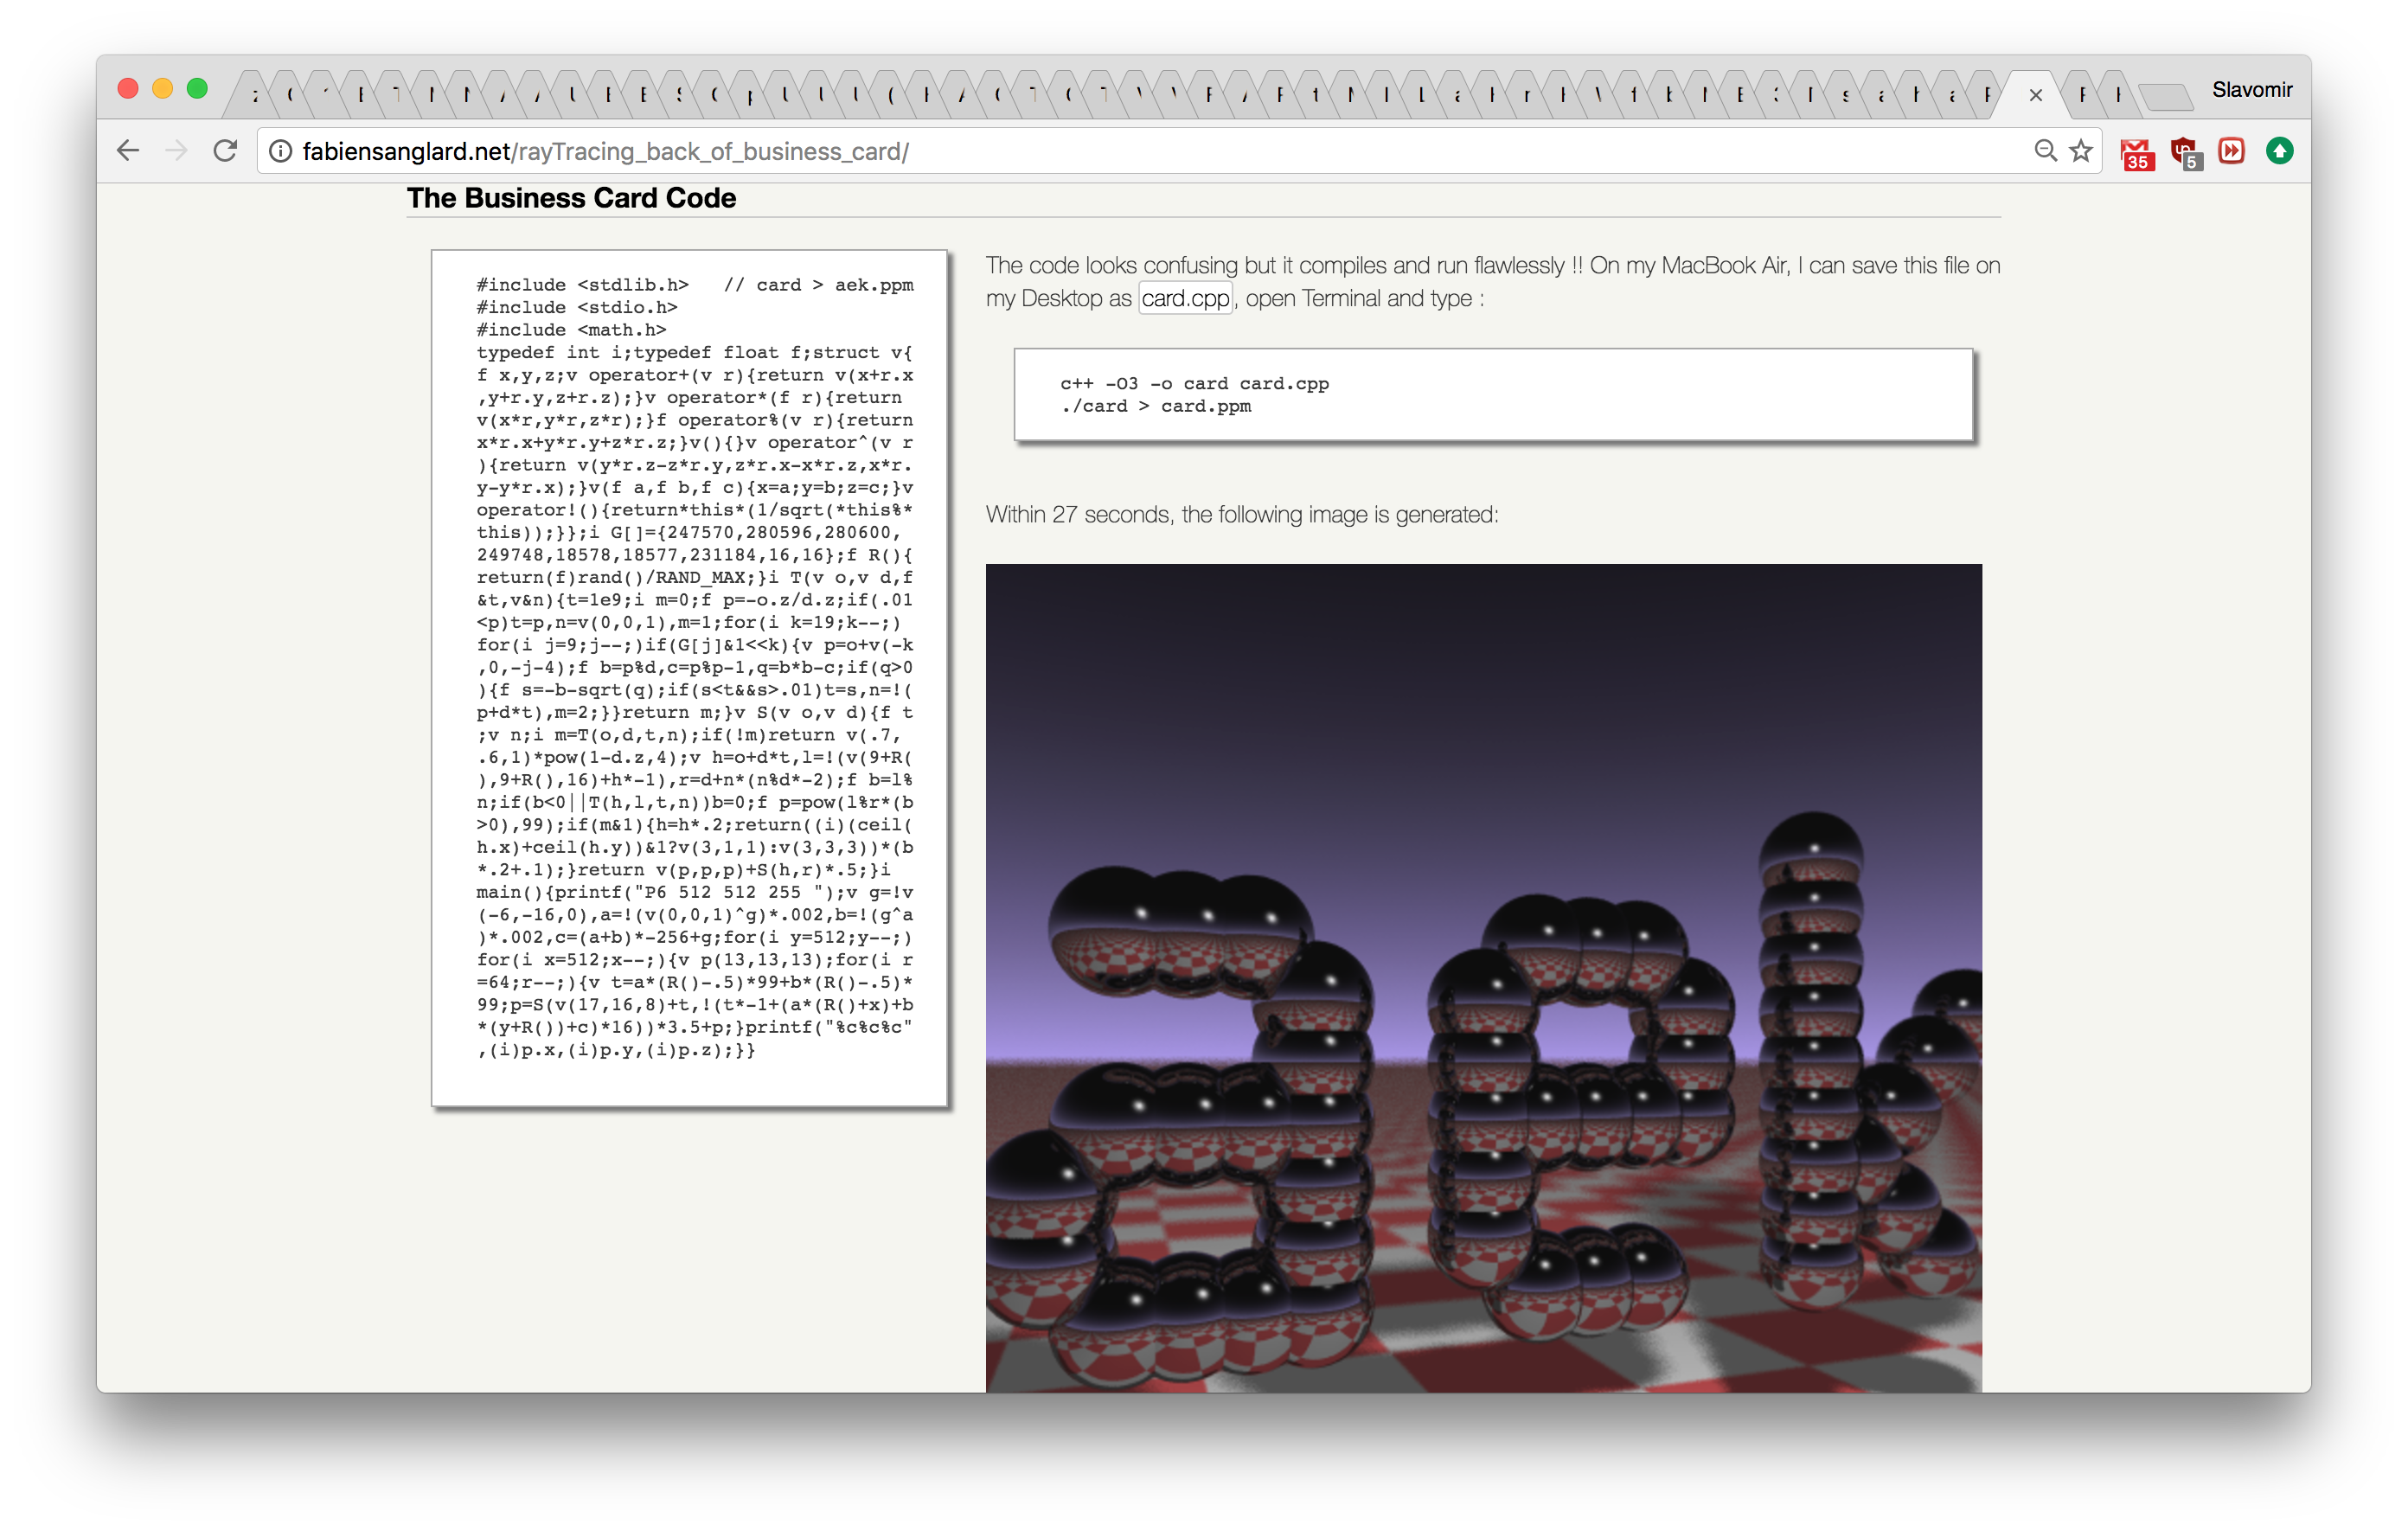
\includegraphics[scale=0.115]{images/card}
\end{frame}

\begin{frame}{The Rendering Equation}
  \begin{align*}
    L(p, \omega_o) = L_e(p, \omega_o) + \int_{S^2} f(p, \omega_o, \omega_i) L(t(p, \omega_i), -\omega_i) \left| \cos \theta_i \right| d \omega_i
  \end{align*}
\end{frame}

\begin{frame}{Analytical solution: Operator formulation}
  \begin{itemize}
    \pause
  \item The light transport operator
    \begin{align*}
      L = L_e + \boldsymbol T L
    \end{align*}
    \pause
  \item What is the solution?
    \pause
    \begin{align*}
      (\boldsymbol I - \boldsymbol T) L & = L_e \\
      L & = (\boldsymbol I - \boldsymbol T)^{-1} L_e
    \end{align*}
    \pause
  \item Power series representation: $L = L_e + \boldsymbol T L_e + \boldsymbol T^{2} L_e + ...$
    \pause
    \begin{align*}
      L & = \sum_{n=0}^{\infty} \boldsymbol T^{n} L_e
    \end{align*}
    \pause
  \item The solution operator
    \begin{align*}
      \boldsymbol S & = (\boldsymbol I - \boldsymbol T)^{-1} \\
      L & = \boldsymbol S L_e
    \end{align*}
  \end{itemize}
\end{frame}

\begin{frame}{Numerical solution: Integral over paths}
  \small
  \begin{align*}
    L(p^{\prime} \to p) = L_e(p^{\prime} \to p) + \int_{A} f(p^{\prime\prime} \to p^{\prime} \to p) L(p^{\prime\prime} \to p^{\prime}) G(p^{\prime\prime} \leftrightarrow p^{\prime}) d A(p^{\prime\prime})
  \end{align*}
  \normalsize
\end{frame}

\begin{frame}{Generating paths}
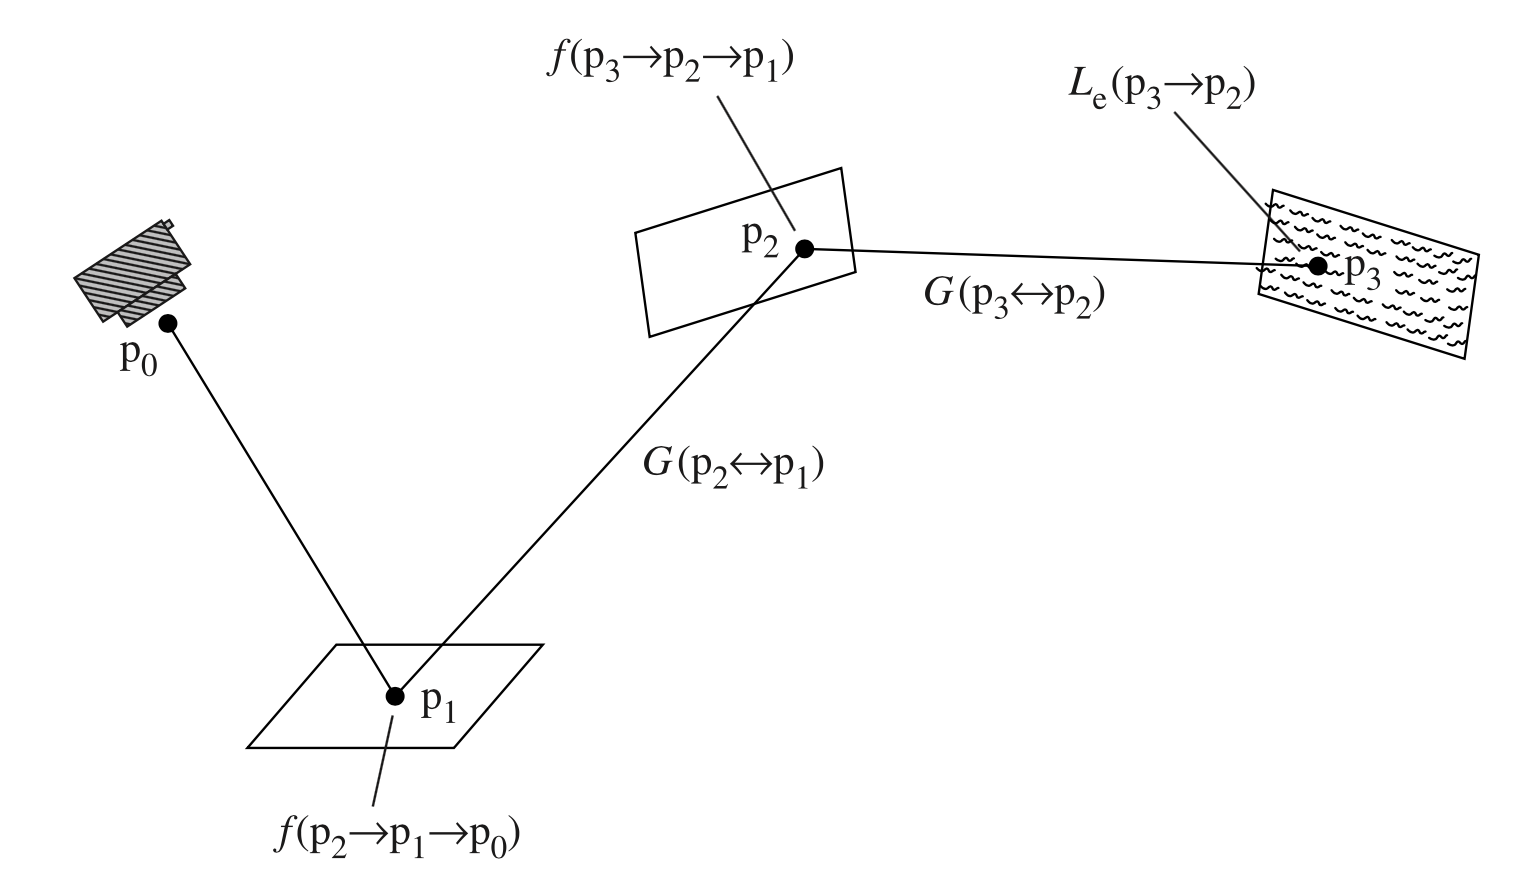
\includegraphics[scale=0.4]{images/paths}
\end{frame}

\begin{frame}{Strategies for generating paths}
  \begin{itemize}
    \pause
  \item Light tracing
    \pause
  \item Path tracing
    \pause
  \item Bidirectional path tracing
    \pause
  \item Vertex connection and merging (VCM)
    \pause
  \item Still an active topic of research
  \end{itemize}
\end{frame}

\begin{frame}{Monte Carlo method}
  \begin{itemize}
    \pause
  \item Monte Carlo methods are a broad class of computational algorithms that rely on repeated random sampling to obtain numerical results
    \pause
  \item Enrico Fermi first experimented with the Monte Carlo method while studying neutron diffusion in the 1930s
    \pause
  \item The modern version of the Monte Carlo method was invented in the late 1940s by Stanislaw Ulam
    \pause
  \item Monte Carlo methods were central to the simulations required for the Manhattan Project
  \end{itemize}
\end{frame}

\begin{frame}{Monte Carlo method I}
  Suppose we want to find the value of $I$ where

  \bigskip
  \begin{align*}
    I = \int_{x \in [0, 1]^s} f(x) dx
  \end{align*}
  \bigskip

  \pause
  and also suppose we have a random variable $X \in [0, 1]^s$ with probability density function $p(x)$.

  \pause
  \bigskip
  What can we say about the expected value of $f(X)$?

  \pause
  \bigskip
  Well by definition of expected value we know that
  \bigskip
  \begin{align*}
    \mathbf{E}[f(X)] = \int_{x \in [0, 1]^s} f(x) p(x) dx
  \end{align*}
\end{frame}

\begin{frame}{Monte Carlo method II}
  What about the expected value of $\frac{f(X)}{p(X)}$?

  \pause
  \bigskip
  Let's see

  \begin{align*}
    \mathbf{E}[\frac{f(X)}{p(X)}] &= \int_{x \in [0, 1]^s} \frac{f(x)}{p(x)} p(x) dx \\
    & = \int_{x \in [0, 1]^s} f(x) dx = I
  \end{align*}

  \pause
  \bigskip
  Therefore

  \begin{align*}
    I = \mathbf{E}[\frac{f(X)}{p(X)}]
  \end{align*}
\end{frame}

\begin{frame}{Monte Carlo method III}
  \pause
  The general idea is to approximate the integral we're interested in
  \begin{align*}
    I = \int_{x \in [0, 1]^s} f(x) dx
  \end{align*}
  \pause
  by a sum
  \begin{align*}
    \widetilde{I_N} = \frac{1}{N} \sum_{i=1}^{N}{\frac{f(x_i)}{p(x_i)}}
  \end{align*}
  \pause
  It can be shown that $\widetilde{I_N}$ is an unbiased estimator of $I$ which
  converges to the correct value as $N \to \infty$
  \pause
  \begin{align*}
    \mathbf{E}[\widetilde{I_N}] & = I \\
    \mathbf{V}[\widetilde{I_N}] & = \frac{1}{N} \mathbf{V}[\frac{f(X)}{p(X)}] \\
    \sigma[\widetilde{I_N}] & = \frac{1}{\sqrt{N}} \sigma[\frac{f(X)}{p(X)}]
  \end{align*}
\end{frame}

\begin{frame}{Random Numbers: xkcd \#221}
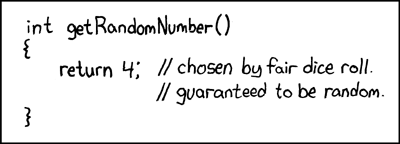
\includegraphics[scale=0.77]{images/xkcd221}
\end{frame}

\begin{frame}{Quasi-Monte Carlo Method}
  \begin{outline}
    \pause
  \1 The Koksma-Hlawka inequality
  \begin{align*}
    \left| \widetilde{I_N} - I \right| \leq \mathbf{V}[f] D_N^{*}(x_1, ..., x_N)
  \end{align*}
    \pause
  \1 Roughly speaking the star discrepancy of a point set $D_N^{*}(x_1, ..., x_N)$ is a
    measure of how uniformly the sequence $x_1, ..., x_N$ is distributed in $[0, 1]^s$
    \pause
  \1 The main discrepancy conjecture
  \begin{align*}
    D_N^{*}(x_1, ..., x_N) \geq c_s \frac{(\ln{N})^{s}}{N}
  \end{align*}
    \pause
  \2 Proved for $s \leq 2$ by W. M. Schmidt. The problem is stil open in higher dimensions.
    \pause
  \1 Low discrepancy sequences: van der Corput, Halton, Hammersley, Sobol and others
  \begin{align*}
    D_N^{*}(x_1, ..., x_N) \leq C \frac{(\ln{N})^{s}}{N}
  \end{align*}
  \end{outline}
\end{frame}

\begin{frame}{Let's design a sampler: fract demo}
  \begin{itemize}
    \small
    \pause
  \item Python, NumPy, Z3 Theorem prover
    \pause
  \item Z3 is an open source Satisfiability Modulo Theories (SMT) solver by Microsoft Research
    \pause
  \item https://github.com/skaslev/fract/blob/master/mc-production.ipynb
    \pause
  \item https://github.com/skaslev/pyman
  \end{itemize}
\end{frame}

\begin{frame}{Future}
  \begin{outline}
    \pause
    \1 ``It's hard to make predictions, especially about the future.'' \pause Niels Bohr
    \pause
    \1 Faster Monte Carlo convergence
    \pause
    \2 Can we do better than $O(N^{-1/2})$? \pause Maybe. \pause Maybe not.
    \pause
    \2 ``Advanced mathematical methods for scientists and engineers'' by Carl Bender
    \pause
    \1 Noise filtering and machine learning
    \pause
    \1 Better mathematical models
    \pause
    \2 Renderer based on Quantum Electrodynamics (QED) rather than classical approximations
    \pause
    \2 ``QED: The Strange Theory of Light and Matter'' by Richard Feynman
    \pause
    \2 ``Richard Feynman Lecture on Quantum Electrodynamics: QED'' https://www.youtube.com/watch?v=LPDP\_8X5Hug
    \pause
  \end{outline}
\end{frame}

\begin{frame}{The Feynman Algorithm}
  \pause
  \begin{itemize}
  \item Write down the problem
    \pause
  \item Think real hard
    \pause
  \item Write down the solution
  \end{itemize}
\end{frame}

\begin{frame}{$A x = b$}
  \pause
  \begin{itemize}
  \item Write down the problem
    \pause
  \item Rewrite the problem as $A x = b$
    \pause
  \item Use off the shelf solver or write a specialized one
  \end{itemize}
    \pause
  ``All problems in computer graphics can be solved with a matrix inversion.'' Jim Blinn
\end{frame}

\begin{frame}{Eigenvalue problems}
  \pause
  \begin{itemize}
  \item Write down the problem
    \pause
  \item Rewrite the problem as $A x = \lambda x$
    \pause
  \item Use off the shelf solver or write a specialized one
  \end{itemize}
\end{frame}

\begin{frame}{Perturbation theory}
  \begin{itemize}
    \pause
  \item Write down the problem
    \pause
  \item Insert a ``small'' parameter $\epsilon$ in so that the problem is trivial when $\epsilon = 0$
    \pause
  \item Guess the solution has the form $x = \sum_{n=0}^{\infty}{a_n \epsilon^n}$
    \pause
  \item Plug that back in the equation and solve for $a_n$
    \pause
  \item Sum the series and substitue $\epsilon = 1$
  \end{itemize}
\end{frame}

\begin{frame}{Further reading}
  \small
  \begin{itemize}
  \item ``Physically Based Rendering: From Theory to Implementation'' by Matt Pharr and Greg Humphreys
  \item ``Robust Monte Carlo Methods for Light Transport Simulation'', Eric Veach, Ph.D. dissertation
  \item ``Light Transport Simulation with Vertex Connection and Merging'' by Iliyan Georgiev, Jaroslav Křivánek, Tomáš Davidovič, Philipp Slusallek
  \item ``Random Number Generation and Quasi-Monte Carlo Methods'' by Harald Niederreiter
  \item ``Quantum Mechanics and Path Integrals'' by Richard Feynman
  \item ``An Introduction to the Analysis of Algorithms'' by Robert Sedgewick and Phillipe Flajolet
  \item ``Mathematical Physics'', Carl Bender, https://www.youtube.com/watch?v=LYNOGk3ZjFM
  \item ``fract'', source code from this presentation, https://github.com/skaslev/fract
  \end{itemize}
\end{frame}

\begin{frame}{Questions?}
\end{frame}

\begin{frame}{Thank you}
\end{frame}

\end{document}
